\section{Le conte, vecteur de transmission d'humanisme en déclin}

\begin{shadequote}
Le premier véritable récit est et demeure le conte. \par\emph{Walter Benjamin, Der Erzähler}
\end{shadequote}

%\begin{figure}[h!]
%    \centering
%    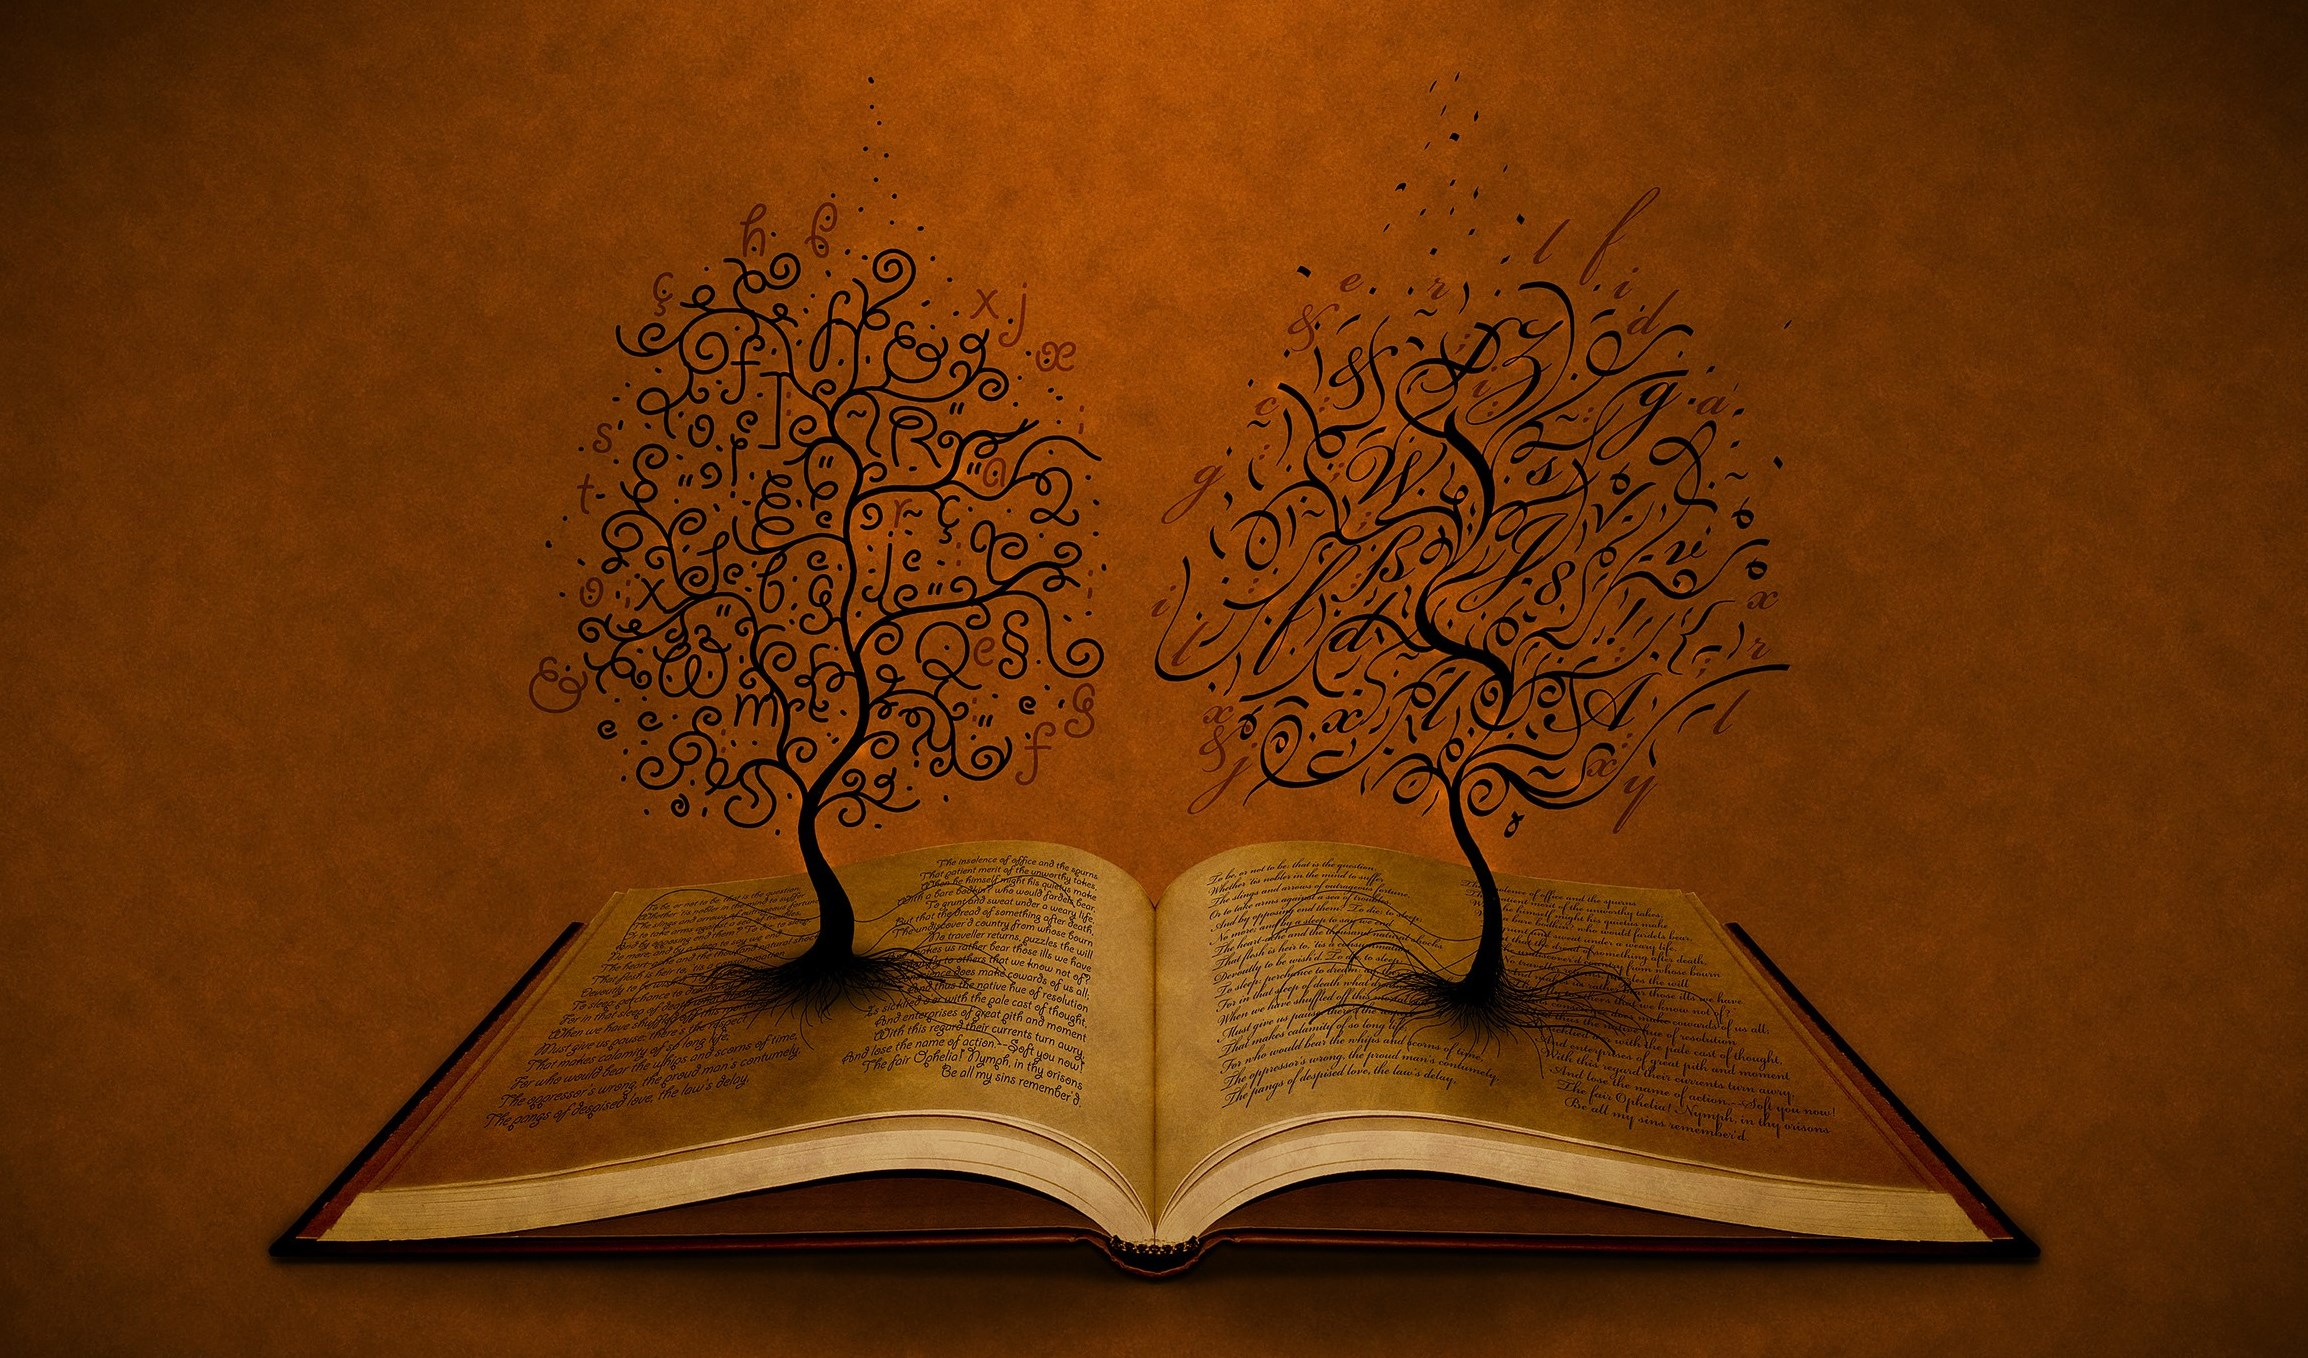
\includegraphics[width=0.80\linewidth]{img/tale_book.jpg}
%    \caption{Tale book}
%\end{figure}

\subsection{Vecteur d'expérience}
Dans ses origines, lesquelles se perdent dans l'histoire de l'humanité, et encore aujourd'hui, le conte oral est considéré comme un vecteur destiné à perpétuer l'expérience d'un vécu et renouveler la tradition portée par ses conteurs. Ces contes, que l'on peut associer à une littérature orale où le conteur endosserait un rôle de narrateur, s'opposent originellement aux mythes car voués à « rapporter à quelqu'un un fait réel »\cite{cnrtl}.

On notera alors deux figures emblématiques du conteur ; d'une part un personnage sédentaire, d'autre part un voyageur. Le premier perpétue un « lointain temporel »\cite{nouss2003conteur}, c'est-à-dire une histoire riche d'expériences passées et transmise à travers les générations. On associera donc naturellement ces êtres à la mémoire d'un peuple, gardiens de la tradition et du savoir des générations passées. Le second parcourt ce monde à la recherche de rencontres humaines et d'échanges culturels, ce dans le but de diffuser à tout un chacun un « lointain spatial » \textit{(ibid)}, récits d'expériences vécues ou entendues en d'autres lieux.

Le métier de conteur revêt donc une dimension sociale d'importance, associée à la transmission systématique d'une expérience qui est la teneur principale du conte. Une interprétation probable de la cause d'une perte de vitesse manifeste de la transmission orale via le conte résiderait alors dans la valeur accordée au conte par son public. En effet, l'intérêt porté par les jeunes générations à l'expérience serait en net déclin, notamment de par l'omniprésence de l'information journalistique à travers une multitude de médias. Cette information rapportée notifiant son public captif des derniers évènements survenus, analysés et expliqués, elle s'oppose magistralement au conte, ce dernier laissant à son auditoire le soin d'une réflexion visant à une interprétation propre accompagnée de ses conclusion. Le conte délivre en effet un fait nu, valorisant le processus intellectuel de son public.

La valeur des contes ne résiderait donc pas dans leur intrigue, mais dans la mise en valeur de l'acte qu'est le vécu d'une expérience. Les contes véhiculent ainsi une conception de l'être humain et de la vie, celle de vivre des expériences, de traverser des épreuves, et de les surmonter.

On notera enfin une dérive du genre à travers l'époque contemporaine, les récits véhiculés ne faisant plus nécessairement référence à un vécu réel, mais plus souvent « brodé » ou façonné, néanmoins souvent porteur d'une morale visant à enrichir son auditoire.

%\begin{figure}[h!]
%    \centering
%    
\includegraphics[width=0.80\linewidth]{img/storyteller.png}
%    \caption{Storyteller}
%\end{figure}

\subsection{Un processus d'attention flottante}

\begin{shadequote}
[...] en conformant son choix à son expectative, on court le risque de ne trouver que ce que l'on savait d'avance.
\par\emph{Walter Benjamin, Der Erzähler}
\end{shadequote}

Dans l'écoute du conte, le procédé freudien d'attention flottante \cite{freud1996ratschlage} consistant en l'absence d'attention dirigée ou focalisée, permettrait à l'auditeur de s'oublier lui-même, afin que «les mots qu'il entend[e] s'inscrivent profondément en lui» (\cite{benjamin1991gesammelte}), facteur essentiel de l'assimilation et de la mémorisation des contes par l'auditoire via une écoute détendue.\\

Favorise la libre association des idées
Les psychanalyse l'utlisaient pour interpréter ce que leur rapportait leur patient (au lieu de noter)

conserver dans sa mémoire une multitude d'éléments en apparence insignifiants dont les corrélations ne ressortiront qu'ultérieurement.

\subsection{De l'autorité mortuaire}

\begin{shadequote}
Le parfait récit naît de l'accumulation de ses versions successives. \par\emph{Walter Benjamin, Der Erzähler}
\end{shadequote}

Chaque conteur apose en effet sa marque au récit, transformant celui-ci de par son vécu.\\
L'existence d'un conte réside dans la mémoire de son auditoire, sa survie dans la transmission perpétuée par ses conteurs. Un conte meurt s'il n'est pas transmis.\\
Une cause cause annexe de déclin pourrait résider dans la conception de la mort par l'humain.\\
Selon W. B., le conteur tient de la mort son autorité. En effet, les contes étant faits de vécu, une vie d'expériences fondera donc une sagesse ou un savoir dont la transmission sera d'autant plus riche que la vie en fut emplie :  «La mort est la sanction de tout ce que relate le conteur» (ibid). À l'heure de sa mort, toute personne devient donc digne d'être écoutée.\\

Le siècle dernier aurait néanmoins bouleversé la conception sociale de la mort dans nos moeurs. Les progrès technologiques et les atrocités commises ont eu pour effet l'acceptation de la conception d'une mort en masse (Hiroshima), pleine de souffrances (camps de déportation), banalisée et quotidienne (médias).\\
La mort étant transformée, l'autorité qu'on en retire en tant que conteur en est également impactée.\\
Les évènements passés ayant bouleversé le rapport mort/vie, ceux-ci ont également impacté la conception que tout un chacun se fait de la survie. La mort d'un être humain conte revêt alors une importance bien moindre, de même que celle d'un conte.

\clearpage
